\chapter{Introduction}
\label{intro}

This chapter gives a background into the motivation behind the
development of the \agentj~framework.  There is an accompanying 
manual \cite{p2psx}, which describes a use of the \agentj~framework
for simulating P2P networks within the NS2 \cite{ns2} 
simulation environment.  \agentj~provides uses with the ability of 
simulating both real-world Java applications within NS2. It
supports a subset of the common transport protocols used by 
applications e.g. UDP, TCP, Multicast etc and enables these 
protocols to be used within NS2 as if the application was running within the
real Internet.  The focus for \agentj~is to simplify the process of 
simulating applications within Ns2 and therefore native familiar 
Java interfaces are provided so that the application only has
to undergo minimal changes in order to be simulated within NS2. 

\agentj~also supports C++ applications but the applications would
have to program to the interfaces we provide via the PAI or Protolib 
toolkits.  Unlike the \agentj~Java implementation the C++ are not 
the same as the native socket implementations and therefore recoding 
would be required. In Java, an application simply needs to change 
package name  to use \agentj, and the interfaces to UDP/TCP 
thereafter are identical.  Therefore, often a find/replace on "java.net" to
"pai.net" suffices and a Java application can be simulated using 
\agentj~within NS2.  We prove by providing the P2PS 
implementation, which works exactly in this way.  P2PS remains the 
same but we've plugged in the \agentj~communications layer.

\section{Motivation for \agentj}


The main developer of \agentj 
\footnote{Ian Taylor, email: ian.j.taylor@cs.cardiff.ac.uk} is working with
the Scalable, Robust Self-Organizing Sensor (SRSS) systems 
group in NRL, which is investigating and modelling, using network 
simulation tools, lightweight network application discovery mechanisms 
suitable for application in mobile sensor systems.  The mobile sensors 
are envisioned to leverage self-organizing computer communication 
networks based on Mobile Ad-hoc Networking (MANET) routing 
protocols which operate using wireless communication links and 
have no centralized administration or control. 

\index{SRSS Group}
\index{MANET}

Each node in a MANET network participates in the discovery of a route 
and therefore low-level routing protocols are paramount to the overall 
behaviour.  However, it is anticipated that middleware network services 
beyond routing will be required to facilitate autonomous self-organization 
of sensors and their various related data collection, processing, 
and reporting functions.  

The complexity of middleware approaches being considered and 
examined range from utilization of simple, organic network services 
which might be provided by the network layer (network name/address 
resolution, IP multicast, ANYCAST) to potentially heavy-weight, 
highly stateful, complex agent-based architectures.  The focus of 
this task will be lightweight (minimally complex) middleware discovery 
mechanisms and services which can facilitate �publish and subscribe� 
relationships among a set of sensor application peers participating 
in an SRSS network.  The context of highly dynamic, possibly mobile, 
networking will place special challenges on such protocols� ability to 
perform peer neighbor and service discovery and to maintain that 
information in the face of node outages and/or relocation 
within the network.  

\subsection{Investigation into P2P}
 
To satisfy these goals, the SRSS project has been looking into the use of 
lightweight peer-to-peer (P2P) solutions for dynamically discovering 
and connecting the mobile sensor nodes.    P2P middleware attempts 
to create a virtual overlay \cite{overlay} over the existing Internet 
to enable collaboration and sharing of resources. Further, recent 
P2P approaches have been designed to connect individual users 
using highly transient  devices and computers living at the edges of the 
Internet (i.e., behind NAT, firewalls etc) \cite{shirky}.  Therefore, 
\agentj~provides the framework and other systems e.g. P2PS, 
provide the P2PS techniques that run within NS2 using \agentj. For
a discussion of why P2PS was chosen instead of other middleware
approaches (e.g. Jxta), see \cite{p2psx}.

The P2P approach is interesting to the SRSS group because 
mobile sensors within wireless networks exhibit similar types of 
behaviour as Internet peers, but are hosted within an even 
more hostile environment; that is, nodes are disappearing/reappearing 
frequently, data rates are continuously changing as the sensors 
move away from the wireless hubs and other factors, such as 
battery strength, which can affect the type of role the sensor can 
play within the network. It could be argued that a mobile sensor 
application working in such an environment provides 
an excellent stress test for the P2PS protocols employed as it is far
more dynamic than a conventional Internet application.  

\subsection{The sensors}

The actual sensors are relatively simple devices that consist of a CPU, a
data collection mechanism e.g. ADC convertor for audio, images etc and
a wireless network card for communication across the MANET network
to other participating nodes in the community.  

\begin{figure}
\centering
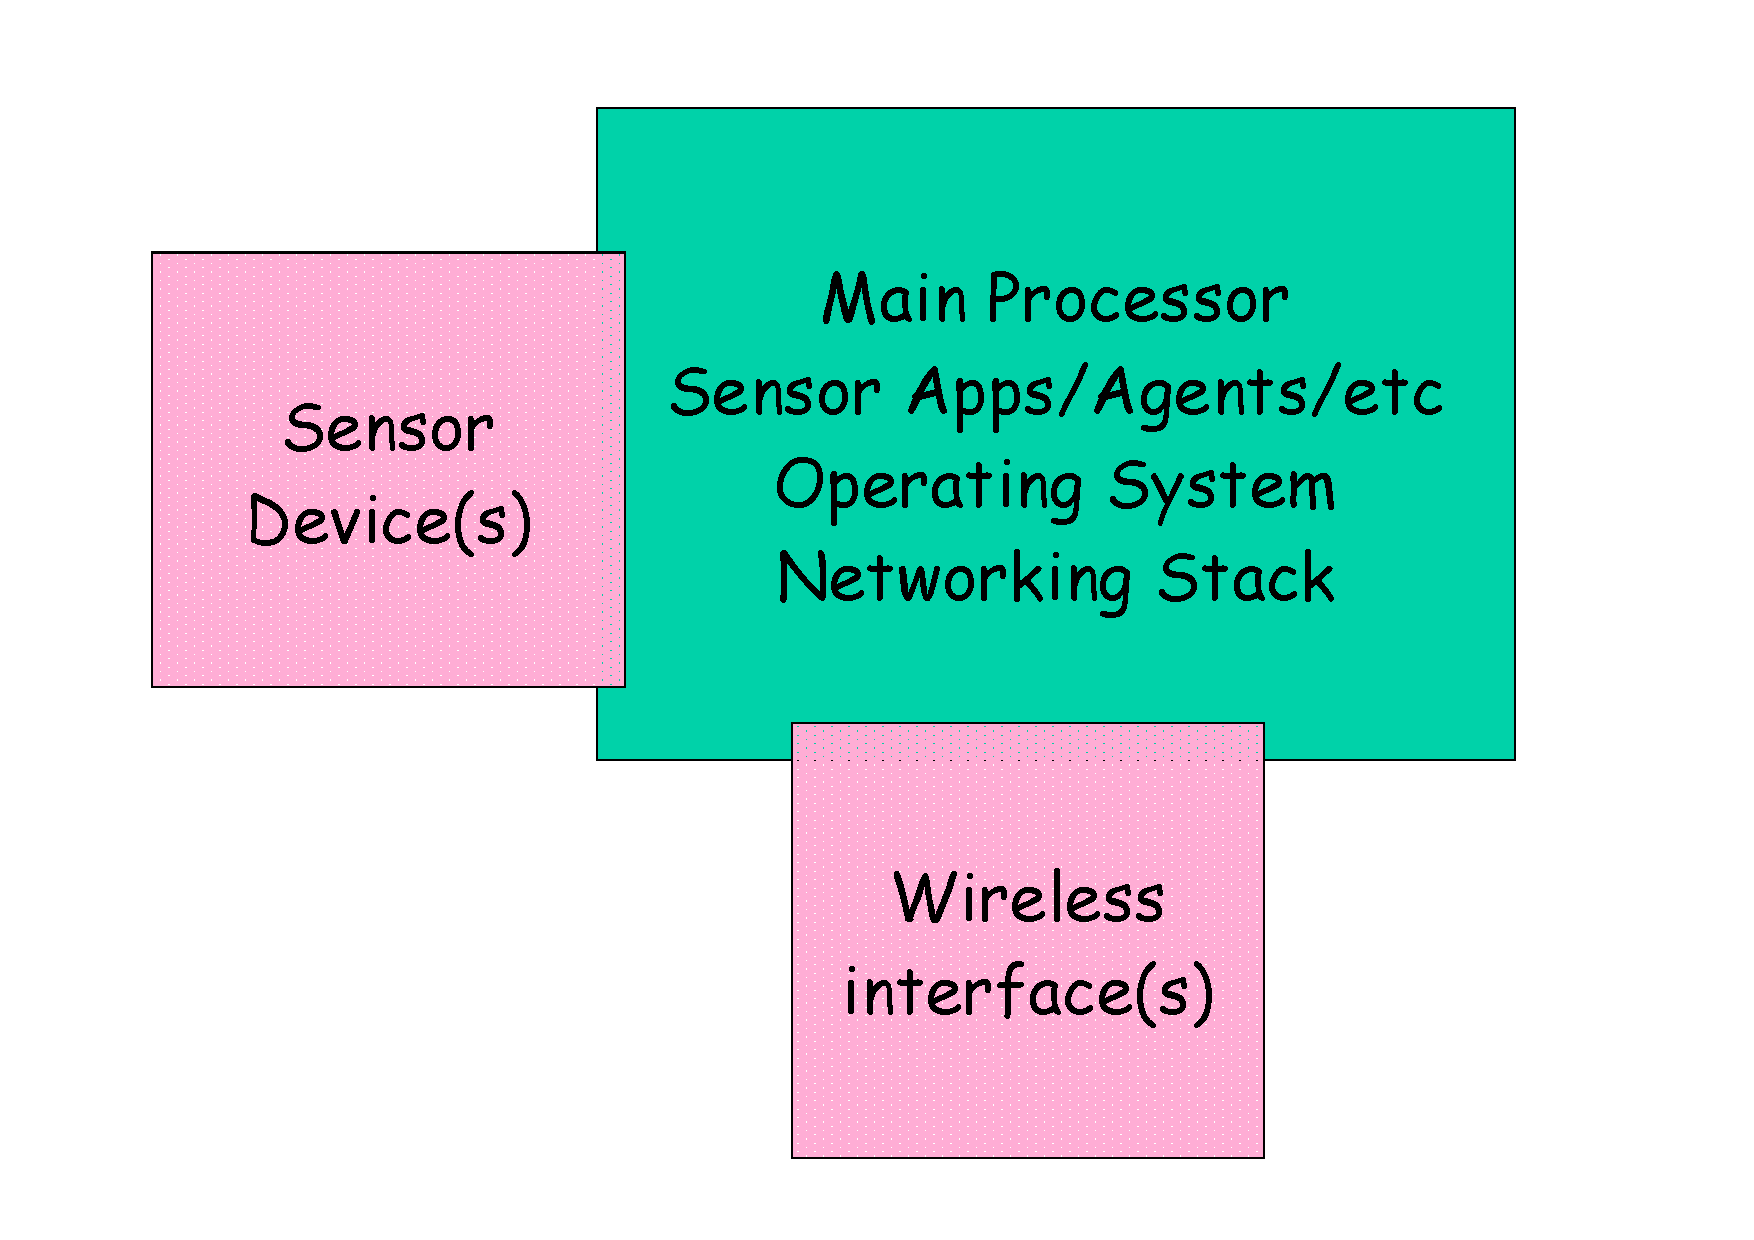
\includegraphics[scale=0.4]{images/introSensor}
\caption{The components of a wireless sensor within an SRSS network.} 
\label{intro:fig:sensor}
\end{figure}


\section{Overview of the \agentj  Architecture}

\agentj~implements a Java framework for plugging in Java applications (e.g.
SRSS mobile node behaviour) and middleware, such as the GAP 
and its bindings e.g. P2PS.  The GAP interface and P2PS middleware 
are described briefly here in Sections \ref{intro:gap} and 
\ref{intro:p2ps} and in detail in the accompanying P2PSx 
manual \cite{p2psx}.

\begin{figure}
\centering
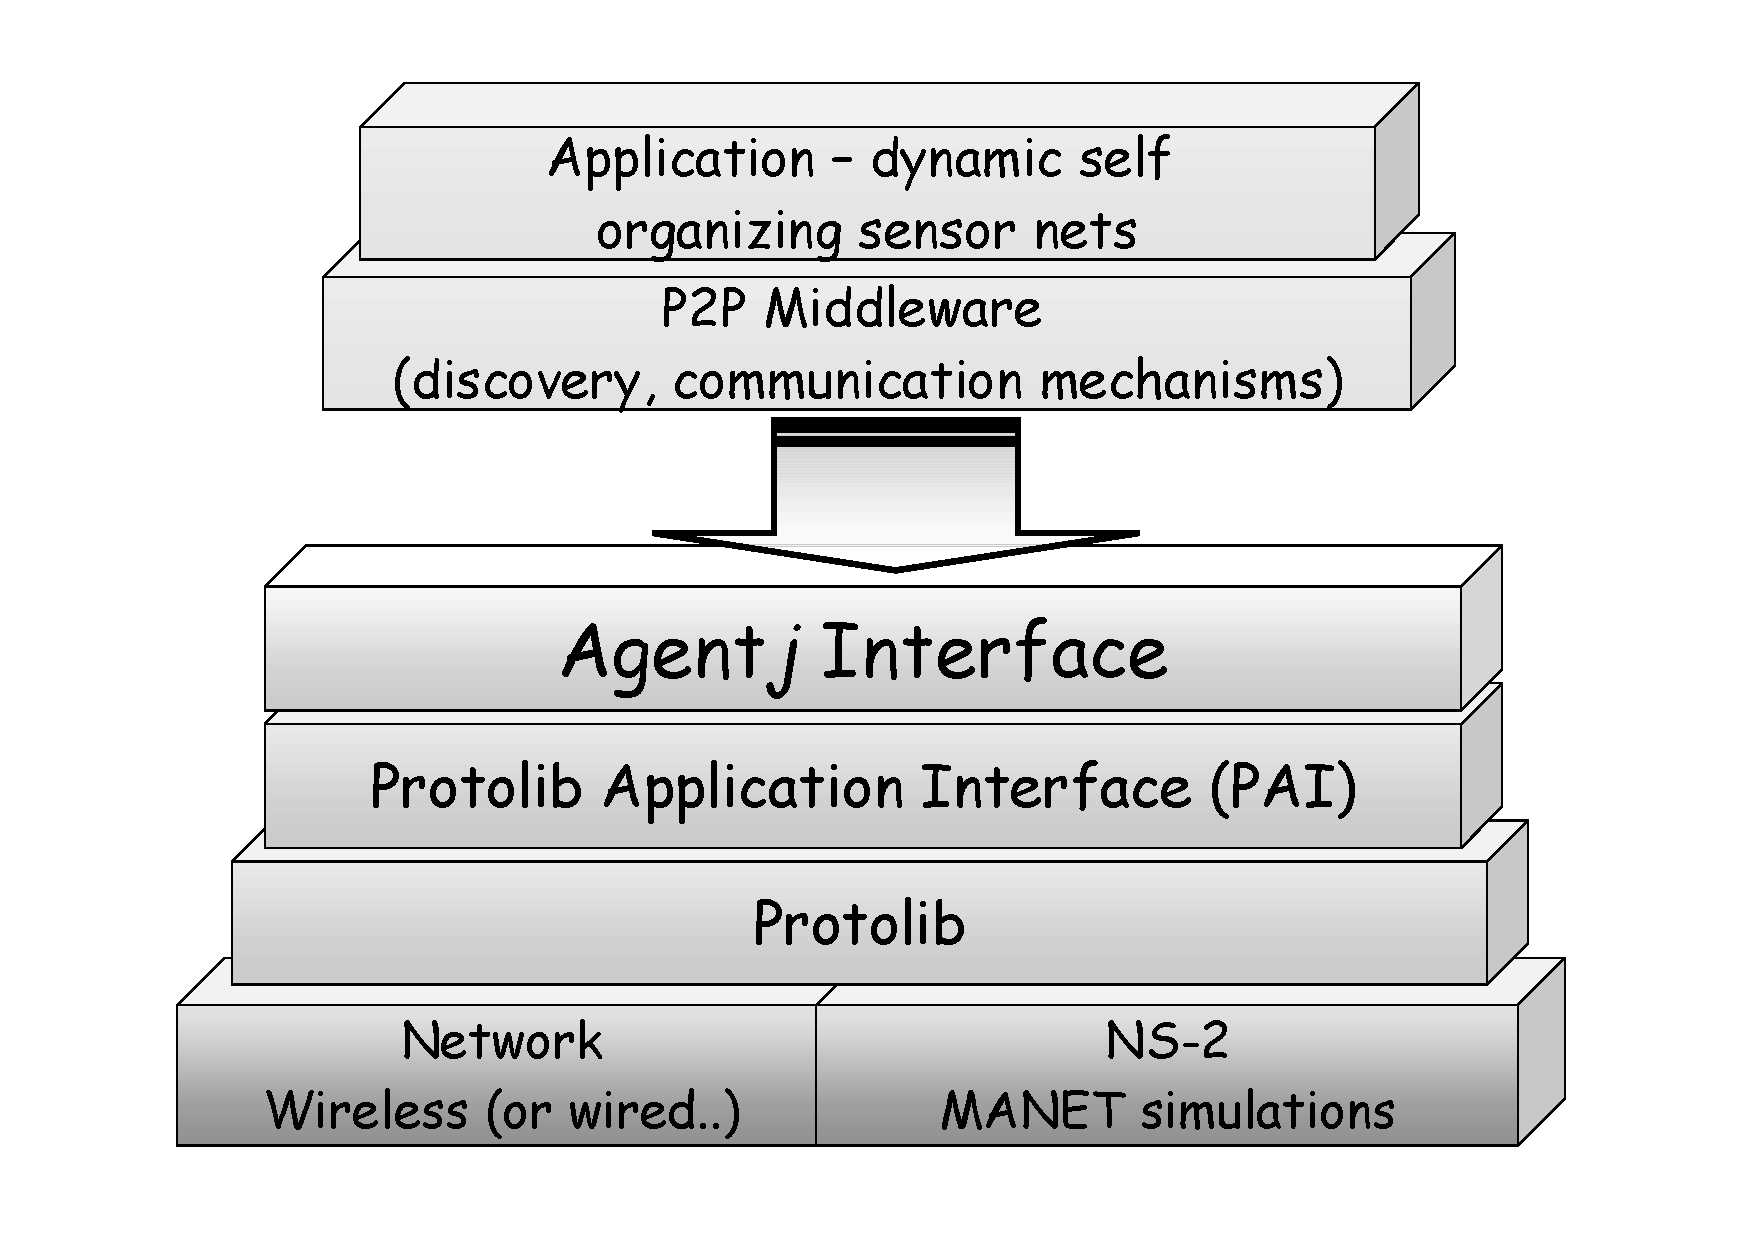
\includegraphics[scale=0.4]{images/introOverview}
\caption{An overview of the \agentj~software stack} 
\label{intro:fig:layers}
\end{figure}

An overview of the \agentj~software architecture is given in Figure
\ref{intro:fig:layers}.  At the lower levels we have two distinct
environmets that \agentj~application can work within: the Internet (or
networked environment) or within the NS2 simulatiojn environment.
Application typically can switch between the nodes and every effort
has been made to make this transition between a simulated 
environment and a real-world deployment as seamless as 
possible.  

NS-2 \cite{ns2} is a discrete event simulator that supports the link layer upwards 
on the OSI stack i.e. the network, transport, session, presentation 
and application layer, respectively. It can support both wired and wireless 
simulations and works on most platforms and therefore satisfies 
the main focus of the project, that is, to test out various 
P2P discovery and communication mechanisms within various 
network extremities.

The toolkit that provides the glue for the communication protocols
and timing interfaces that can enables \agentj~to switch between 
these modes is called Protolib \cite{protolib}.  Protolib
implements a switchable communications layer for several 
communication protocols (e.g. TCP, UDP, Multicast etc) in that
the same programming interface can be used to communicate 
within either environment. To bind to NS2 or a networked 
environment, typically the application just needs to be 
recompiled.  Protolib is described in detail in Chapter 
\ref{protolib}.

\sloppypar The PAI interface (described in Chapt. \ref{pai}) extends the 
functionality/flexibility of Protolib toolkit by allowing multiple
listeners to be attached to sockets or timers. It also provides
convenient interfaces for creating and deleting socket or timing 
instances and implements an engine for providing the necessary 
housekeeping.  In essence, PAI provides a hosting environment
for Protolib to be deployed in Java applications because it fills
in the gap between what Java applications expect and what
the core Protolib toolkit provides.

Finally, \agentj~provides a familiar Java interface, based around the
\emph{java.net} package, to the underlying functionality provided
by the PAI and Protolib interfaces.  Specifically \agentj~implements
a Java Native Interface (JNI) binding for the PAI C++ interface and
then re-implements this functionality within a set of Java classes
that allow Java programmers to use Protolib sockets as if they
were native Java ones.  The next section describes this interaction 
in more detail.

\begin{figure}[htbp]
\begin{center}
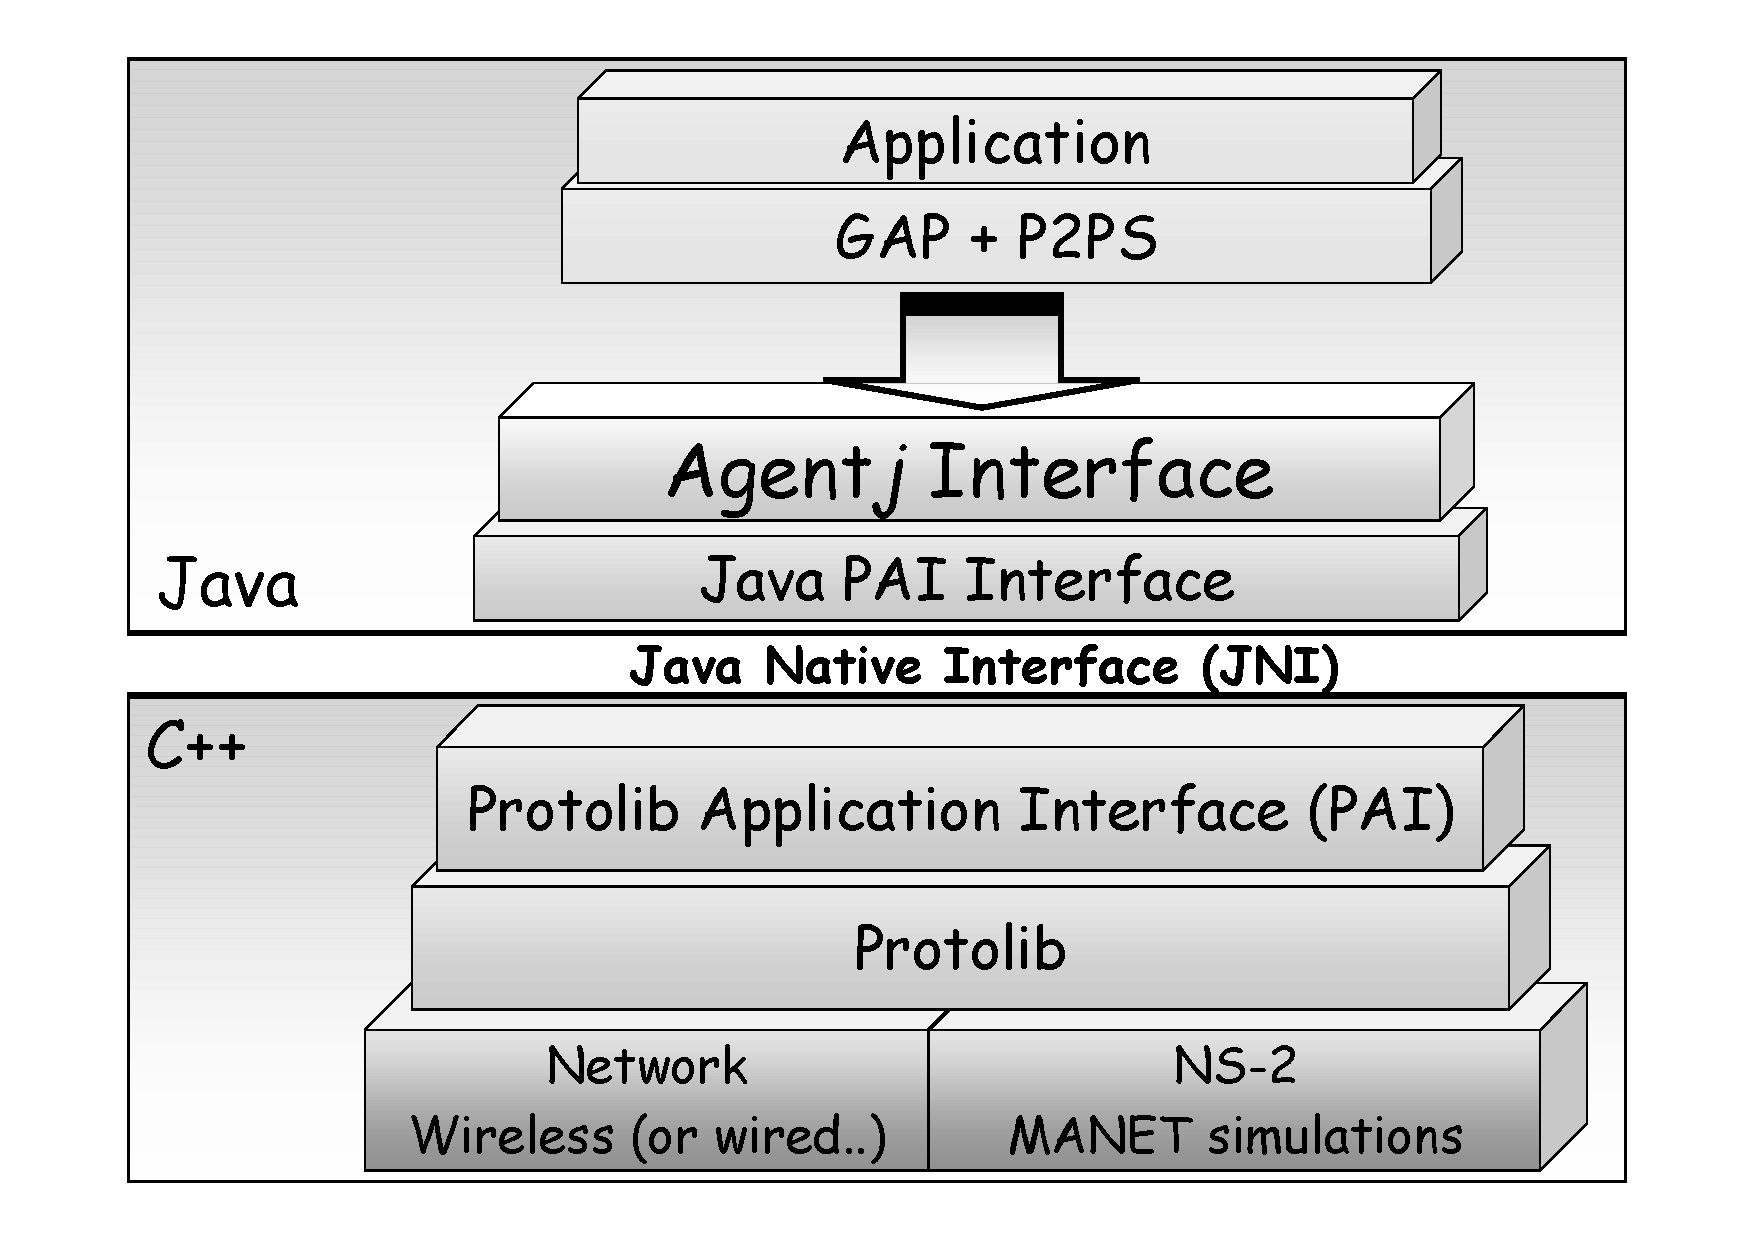
\includegraphics[scale=0.40]{images/introLayers.pdf}
\caption{The \agentj~architecture showing the JNI interface, which provides
the mapping between the NS2 C++ PAI classes and the Java implementation
of the \agentj~interface and applications.}
\label{intro:fig:arch}
\end{center}
\end{figure}

\subsection{\agentj and the JNI PAI Interface}

Since the middleware is written in Java, a JNI bridge is needed in order
to map between the C++ NS2 objects and the associated Java 
objects. This bridging mechanism is required at both the input to
the Java application and at its lower communication layers; that is, 
first the C++ NS2 agents need to access and attach Java 
agents to the NS2 agents, then these Java agents need to be able to
access the PAI C++ interface in order to pass data between NS2
nodes.

In the first case, the C++ agents create a Java Virtual Machine 
(JVM)  in order to create an environment for running and accessing 
Java objects.  In the second case, we provide a mapping
to the PAI and Protolib C++ libraries via the Java PAI interface using 
JNI.  The resulting programming arhictecture is shown in 
Figure \ref{intro:fig:arch}.

In this figure, we show the view from an application developer, 
which illustrates the interface that s/he interacts with.  The
developer of a Java NS2 applications interacts with a set of 
high-level Java classes, whilst this functionality is converted to
a set of Java PAI function calls, which in turn, is converted via
a JNI interface to the C++ PAI interface and down to the Protolib
interface. This interaction is described in more detail 
in Chapter \ref{paiagent}. The next section briefly describes the GAP 
interface and P2PS Middleware and then we summarize the 
complete structure in the final section of this chapter. 

\section{The GAP Interface and P2PS}

\index{P2P Discovery}
\index{GAP}
\index{GAT}

Due to the flexibility needed for comparing different discovery mechanisms 
the SRSS project have adopted the use of a high-level interface, called
the GAP. The GAP is an application-layer interface that has been
been developed at Cardiff University within the Gridlab \cite{gridlab} 
and GridOneD projects \cite{gridoned}. The GAP interface is provides 
access to a core set of advertisement, discovery and communication 
services, which were designed by analysing a number of P2P 
applications and extracting the core functionality most applications 
require.  

\index{SAGA Research Group}

The GAP was motivated by the Grid Application Toolkit (GAT) 
interface \cite{gat}, which is committed to conforming to emerging 
application-level standards that are currently being specified through 
the SAGA  research group at the Global Grid Forum \cite{saga}. The 
GAP provides the asynchronous messaging capabilities for the 
GAT engine, which is currently undergoing widespread adoption 
by many application groups worldwide and featured heavily in
GRIDSTART efforts~\cite{workshop}.

\subsection{The GAT}
\label{sec:gatint}

\index{GAT}

The GAT interface provides a generalised collection of calls to shield Grid
applications from implementation details of the underlying Grid middleware, and
is being developed in the European GridLab project \cite{gridlab}. The 
GAT utilises \emph{adaptors} that provide the specific
bindings from the GAT interface to the underlying mechanisms that implement this
functionality. For example, a \emph{move\_file} command may have many GAT
adaptors that implement this functionality depending upon the particular
execution environment used, such as GridFTP, JXTA pipes or a local \emph{cp}
command. 

GAT may be referred to as \emph{upperware}, which distinguishes it from
middleware (which provides the actual implementation of the underlying
functionality). Until recently, application developers typically interact with
the middleware directly. However, it is becoming increasingly apparent that this
transition from one type of middleware to another is not a trivial one. Using
interfaces like GAT, migrating from one middleware environment to another is
easier, and typically achieved by setting an environment variable.  This is
illustrated in the next section where we have implemented an adaptor to bind to
P2P middleware for operating in P2P environments as well as the Grid
environments supported directly by GridLab. This means that exactly the same
Triana implementation can be used within both environments transparently.

\subsection{The GAP Interface}
\label{intro:gap}

\index{GAP Upperware}

The Grid Application Prototype Interface (GAP Interface) is a generic
application interface providing a subset of the GAT functionality. It is
middleware independent, with bindings provided for different Grid middleware
such as JXTA and Web Services, as illustrated in Figure
\ref{fig:gaparchitecture}. 

\begin{figure}[htbp]
\begin{center}
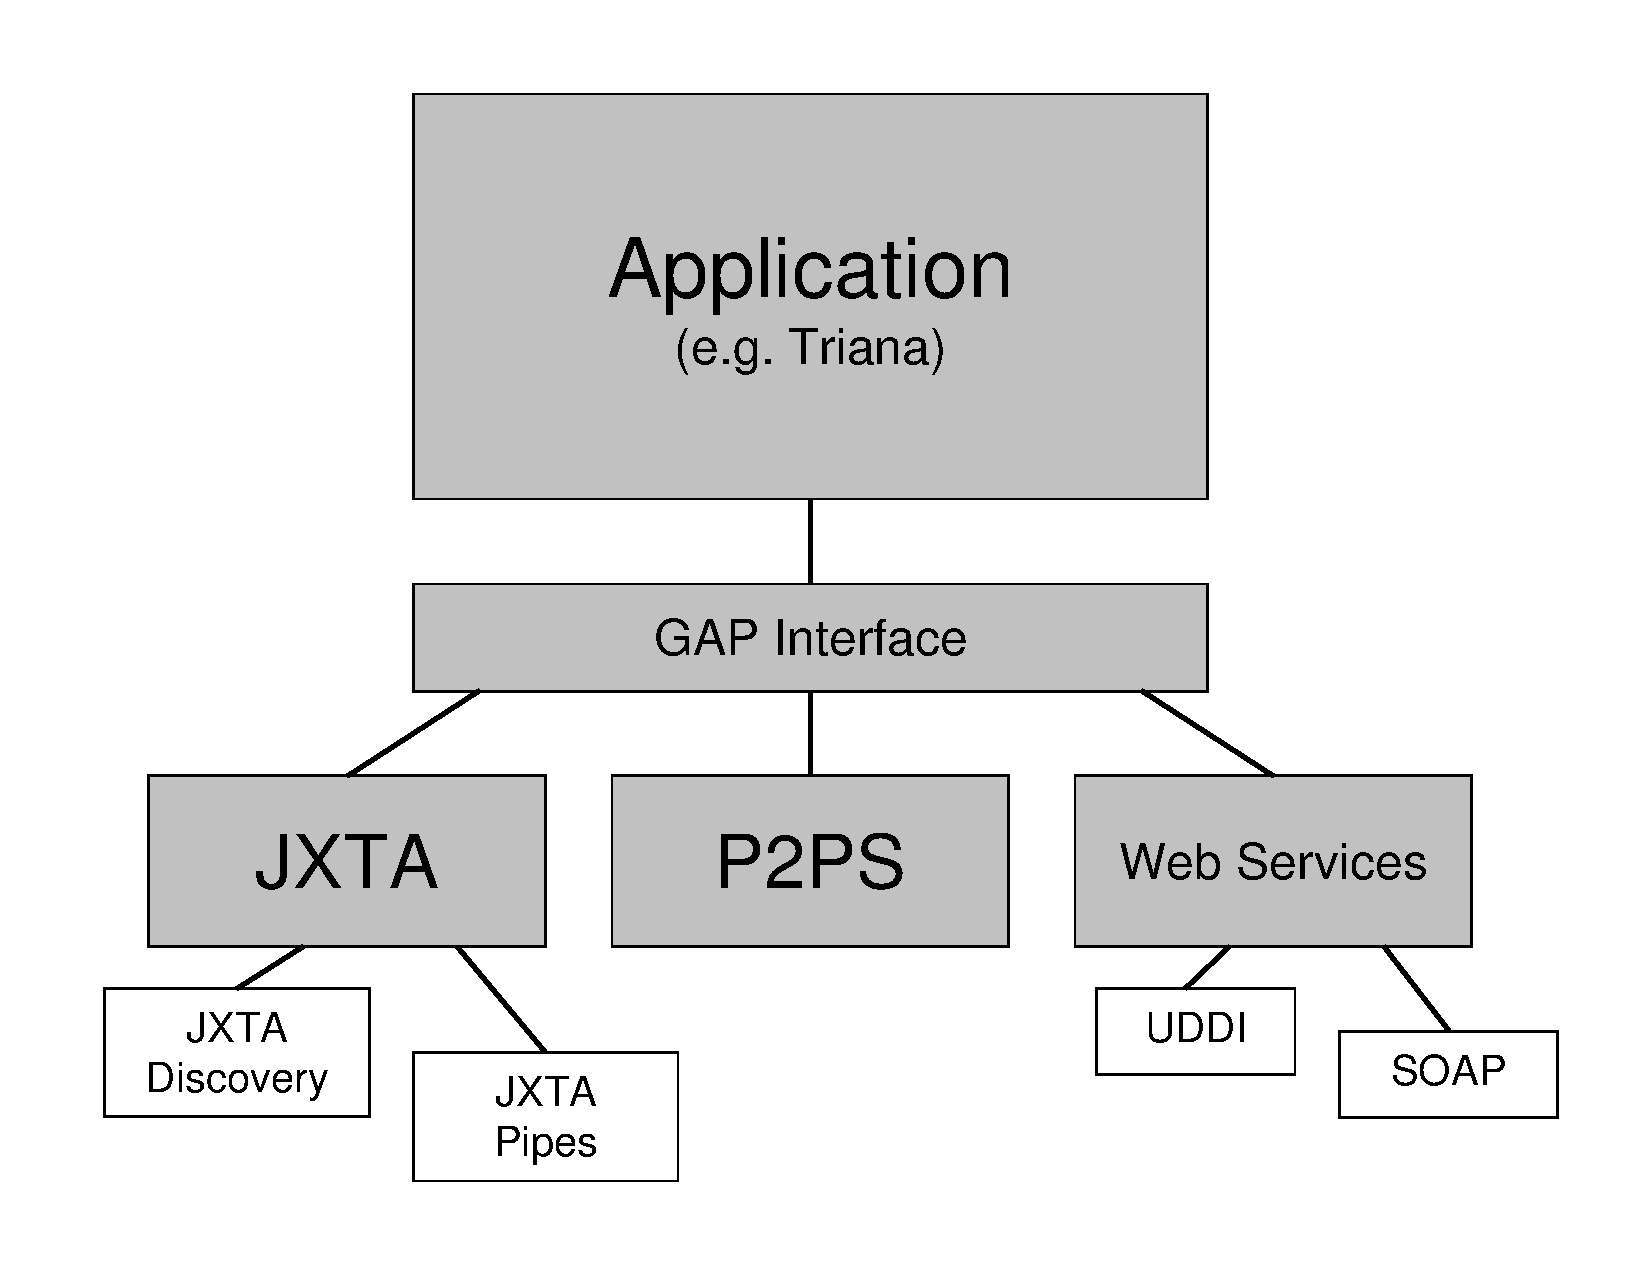
\includegraphics[scale=0.3]{images/gapinterface.pdf}
\caption{The GAP Interface provides a middleware independent
interface for developing Grid applications}
\label{fig:gaparchitecture}
\end{center}
\end{figure}

Part of the motivation behind the GAP Interface is as a stopgap to enable us to
develop distribution mechanisms within Triana while the GridLab GAT is being
developed. When the GridLab GAT becomes available the GAT-API will replace the
GAP Interface within Triana and should enable Triana to make use of the advanced
security, logging and other GridLab services. However, the GAP Interface will
live on, both as a simple interface for prototyping Grid and P2P applications,
and as an adaptor within the GridLab GAT architecture providing various
discovery and communication capabilities. Currently there are three GAP bindings
implemented:

\begin{description}

\item[JXTA] - The original GAP Interface binding was to JXTA~\cite{jxta}. JXTA
is a set of protocols for Peer-to-Peer discovery and communication originally
developed by Sun Microsystems. Although we achieved some initial success with
JXTA, we have since had problems with the speed and reliability of the JXTA
binding. 

\item[P2PS] - a lightweight Peer-to-Peer middleware. See Section \ref{intro:p2ps}
and for a more detailed description, see the P2PSx manual \cite{p2psx}.

\item[Web Services] - The most recent GAP binding allows applications to
discover and interact with Web Services -- using the UDDI registry~\cite{uddi}
and the Web Service Invocation Framework (WSIF)~\cite{wsif}. 

\index{UDDI}
\index{WSIF}
\index{JXTA}
\index{P2PS}

\end{description}

\subsection{P2PS}
\label{intro:p2ps}

P2PS (Peer-to-Peer Simplified) is a lightweight peer-to-peer 
infrastructure. As the name suggests, P2PS aims to provide a simple 
collection of middleware that a develop can use to write peer-to-peer 
style applications, hiding the complexity of other similar architectures 
such as JXTA~\cite{jxta} and JINI~\cite{jini}.

\index{JNI}

Briefly, the P2PS infrastructure is based on XML based discovery and 
communication, which makes it independent of any implementation 
language and computing hardware. P2PS implementations could exist
in any language and there is a specification which can be used to
implement such, although at this time we have only built a prototype
Java implementation. Furthermore, communication within P2PS is 
not tied to any single transport protocol, such as TCP/IP, and 
can be extended to include new protocols, such as Bluetooth or
extend existing ones by writing new endpoint resolvers e.g. we
use this approach to write NS2 endpoint resolvers for TCP and UDP. 

P2PS has been design to operate in highly dynamic, transient 
environments and provides an overlay for discovering anything that
a peer wants to advertise e.g. specific services, rendezvous (caching) peers,
endpoint protocols etc.  P2PS dynamically discovers the capabilities of
other peers at run-time and can negotiate and match how it 
communicates and how it organises its peers.  This makes P2PS
highly suitable for testing out different SRSS discovery mechanisms
for two key reasons.  First, we can test the discovery mechanisms 
built into P2PS (Multicast and Unicast) and secondly, we can easily
extend this to include other protocols by writing new endpoint 
resolvers. Thus, we have a core extensible framework for testing 
and exploring a number of mechanisms both within a simulated 
environment or within a real-world application.

\section{Filling in the Gaps}

\begin{figure}[htbp]
\begin{center}
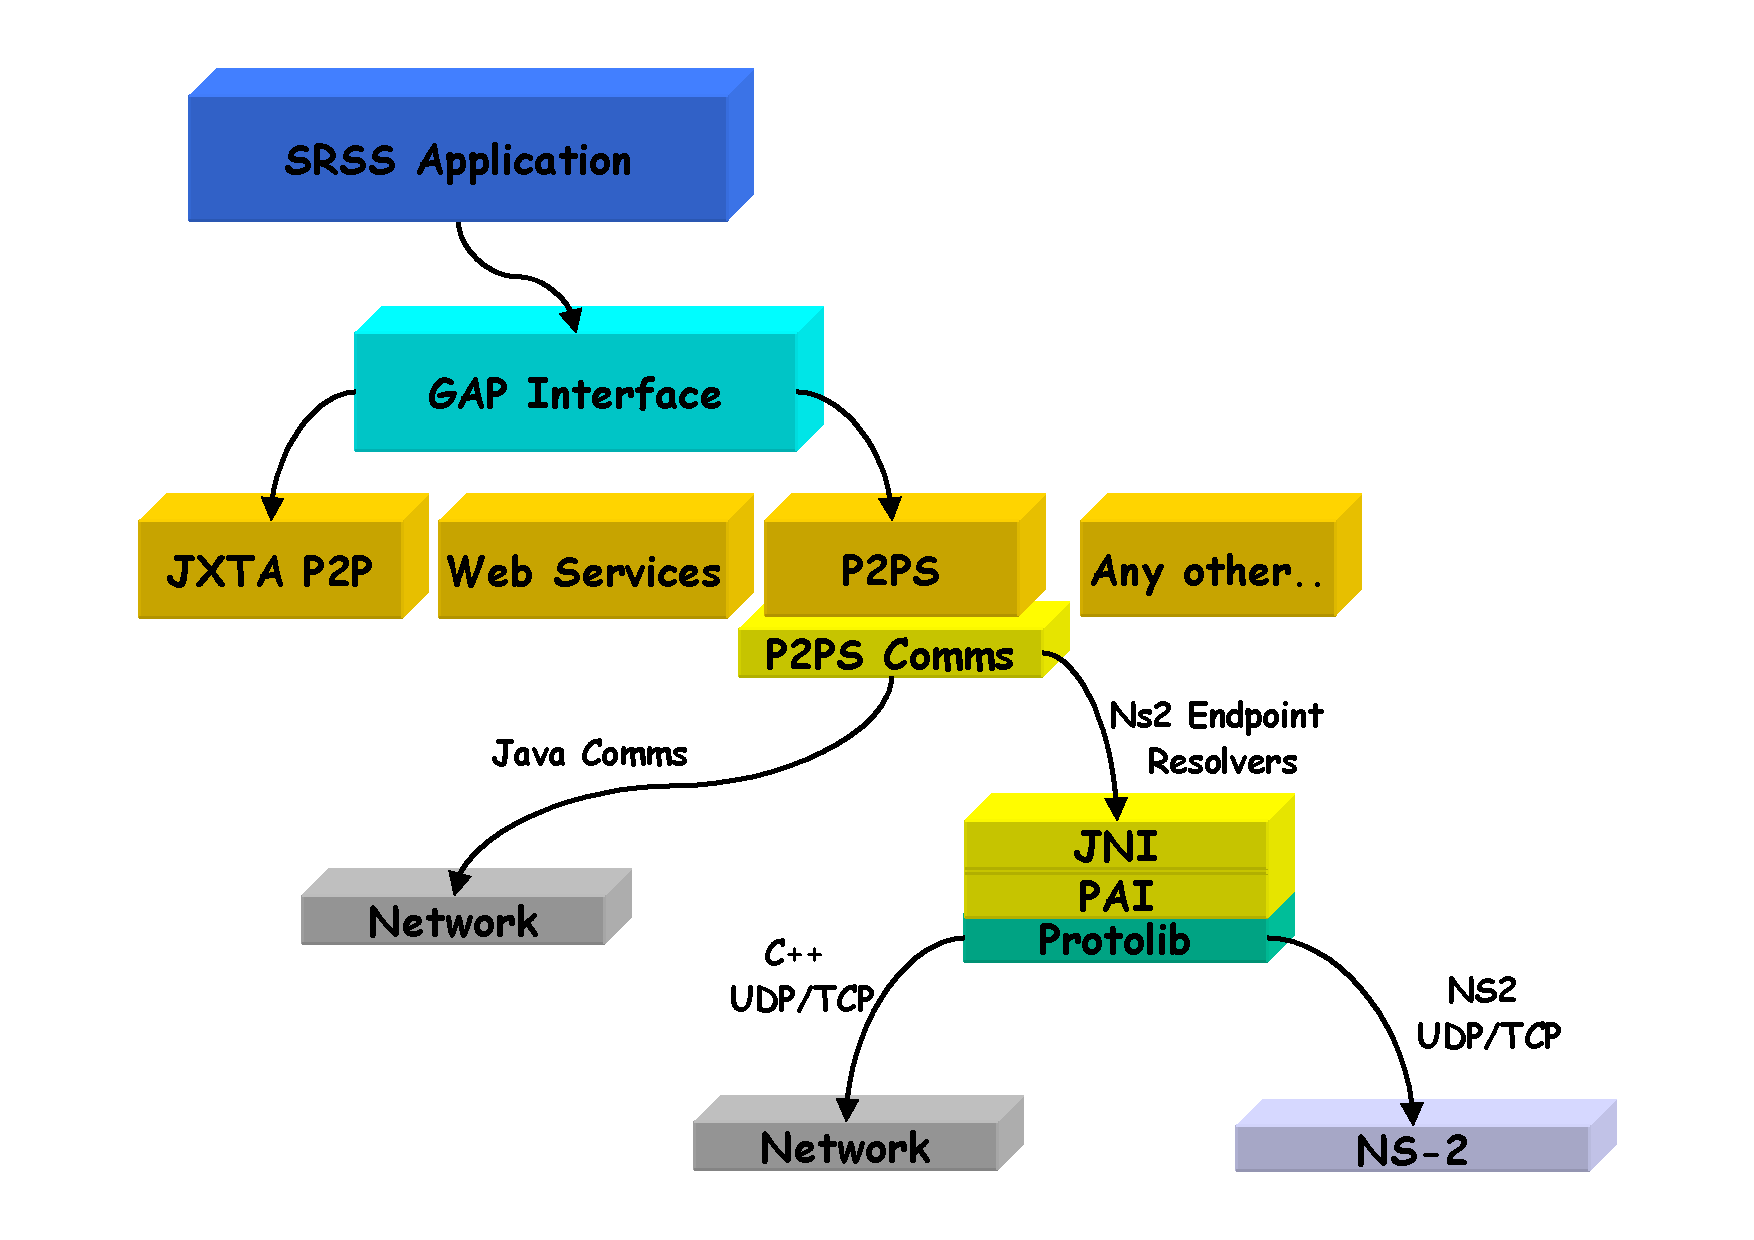
\includegraphics[scale=0.40]{images/introComprehensive.pdf}
\caption{An overview of how the SRSS application will use the complete \agentj~architecture along with the GAP and P2PSx binding.}
\label{intro:fig:comprehensive}
\end{center}
\end{figure}

The resulting architecture is shown in Figure \ref{intro:fig:comprehensive}.  The
application (i.e. mobile sensors) can ulitilise the advertising, discovery
and communication mechanisms provided through the GAP, and also
hook into any of the underlying GAP bindings.

Currently, we have integrated P2PS into NS2 and also we have implemented
a Web services deployment infrastructure using P2PS, allowing 
standardised Web services to be deployed and tested within this 
environment also. This means that any pre-written Web service that
uses WSDL for its interface and communicates using SOAP can be
hosted within NS2 using P2PS.
  
As illustrated in Figure \ref{intro:fig:comprehensive}, P2PS then uses
the Agentj Java socket implementation, which in turn, uses the
Java PAI interface. The Java PAI interface then maps one-to-one with the
C++ PAI interface, which uses Protolib to hook into the lower-level
communication layers.  This enables the resulting
application to be deployed in a networked or an NS-2 simulation
environment.

\section{Conclusion}

In this chapter a background and motivation into the \agentj~project
was given.  We discussed the project that evolved \agentj~and how
the system fits in with their particular research aims and 
objectives.   We then gave an architectural overview of \agentj~and
discussed the various components and interfaces that make up
the entire system.  A summary of each component was given, laying
out the groundwork for the rest of the chapters in this 
manual. 
 



